%=========================================================================
% Start of first day's activities
%=========================================================================
\preClass{Riemann Sums}

\begin{problem}
  \item Determine the value of the integral
  \begin{eqnarray*}
    \int^3_1 f(x) ~ dx,
  \end{eqnarray*}
  where the graph of the function, $f(x)$, is given below.

   \begin{tikzpicture}[scale=2.5]
     \draw[step=1,loosely dotted,line width=1] (-1,-1) grid (4,4);
     \draw[line width=2.2,->] (-1,0) -- (4,0);
     \draw[line width=2.2,->] (0,-1) -- (0,4);
     \begin{scope}
       \clip (0,0) rectangle (2,2);
       \draw[red] (1,0) circle(1.0);
     \end{scope}
     \draw[red] (2,0) -- (3,3);
     \node[left] at (-0.2,3.5) {$f$};
     \node[below] at (3.5,-0.2) {$x$};
     \foreach \x in {-1,1,2,3,4}
        \draw (\x,1pt) -- (\x,-3pt) node[anchor=north east] {\x};
     \foreach \y in {-1,1,2,3,4}
         \draw (1pt,\y) -- (-3pt,\y) node[anchor=north east] {\y};
    \end{tikzpicture}

  \clearpage

  \item Approximate the integral
  \begin{eqnarray*}
    \int^3_1 \ln(x) ~ dx
  \end{eqnarray*}
  using a Riemann sum with 3 rectangles of equal width.

  \clearpage

\end{problem}


\actTitle{Riemann Sums}

\begin{problem}
\item A 5m rod has a charge density given by
  \begin{eqnarray*}
    \lambda_q & = & 5x~\frac{\mathrm{C}}{\mathrm{m}},
  \end{eqnarray*}
  where $x$ is between 0m and 5m.
  \begin{subproblem}
  \item Make a rough sketch of the rod.
    \vspace{4em}
  \item Divide the rod into 5 equal parts, and determine the length of
    each part, and the coordinates for the endpoints.
    \vfill
  \item Determine the charge density at the left endpoint of each part
    of the rod.
    \vfill
    \clearpage
  \item Determine an estimate for the total charge of each part
    assuming that the charge density is roughly constant over each
    part.
    \vfill
    \vfill
  \item Determine an estimate for the total charge in the rod.
    \vfill
    \vfill
  \item Make a sketch of the charge density function, and indicate the geometric relationship between the density and the total charge.
      \vfill
  \end{subproblem}
\end{problem}

\postClass

\begin{problem}
\item Briefly state two ideas from today's class.
  \begin{itemize}
  \item
  \item
  \end{itemize}
\item
  \begin{subproblem}
    \item
  \end{subproblem}
\end{problem}



%=========================================================================
% Start of second day's activities
%=========================================================================
\preClass{Integrals}

\begin{problem}
  \item Determine the value of the following integrals.
    \begin{subproblem}
    \item $\int^5_0 2x ~ dx$
      \vfill
    \item $\int^5_0 2x^2 ~ dx$
      \vfill
    \item $\int^5_0 2x^2 - 2x ~ dx$
      \vfill
    \end{subproblem}
\end{problem}


\actTitle{Integrals}

\begin{problem}
\item A 5m rod has a charge density given by
  \begin{eqnarray*}
    \lambda_q & = & x e^{-x^2}~\frac{\mathrm{C}}{\mathrm{m}},
  \end{eqnarray*}
  where $x$ is between 0m and 5m.
  \begin{subproblem}
  \item Make a rough sketch of the rod.
    \vspace{4em}
  \item Divide the rod into 5 equal parts, and determine the length of
    each part, and the coordinates for the endpoints.
    \vfill
  \item Determine the formula for the charge density on the left
    endpoint of each part from above.
    \vfill
    \clearpage
  \item Determine the sum using sigma notation for the estimate of the
    total charge in the rod.
    \vfill
  \item Express the limit of the sum as an integral.
    \vfill
  \item Determine the amount of charge in the rod.
    \vfill
  \end{subproblem}
\end{problem}

\postClass

\begin{problem}
\item Briefly state two ideas from today's class.
  \begin{itemize}
  \item
  \item
  \end{itemize}
\item
  \begin{subproblem}
    \item
  \end{subproblem}
\end{problem}


%=========================================================================
% Second Day of U-Substitution
%=========================================================================
\preClass{u-Substitution}

\begin{problem}
\item Determine the values of each of the following integrals.
  \begin{subproblem}
  \item $\int^{10}_1 \frac{1}{1+x^2} ~ dx$
    \vfill
  \item $\int^{10}_1 \frac{x}{1+x^2} ~ dx$
    \vfill
  \item $\int^{10}_1 \frac{e^x}{1+e^{x}} ~ dx$
    \vfill
  \end{subproblem}
\end{problem}


\actTitle{Calculating Total Charge}
\begin{problem}
\item A rod has a charge distribution, and the length of the rod is
  2m. The left endpoint is $x=0$m, and the right endpoint is
  $x=2$m. Determine the total charge in the rod for the following
  charge densities.
  \begin{subproblem}
    \item $\lambda_q = \frac{2}{\sqrt{3x+1}}$ C/m
      \vfill
    \item $\lambda_q = \frac{e^x}{1+e^{2x}}$ C/m
      \vfill
    \item $\lambda_q = x\sin\lp 1+x^2\rp$ C/m
      \vfill
  \end{subproblem}
\end{problem}


\postClass

\begin{problem}
\item Briefly state two ideas from today's class.
  \begin{itemize}
  \item
  \item
  \end{itemize}
\item
  \begin{subproblem}
    \item
  \end{subproblem}
\end{problem}


%=========================================================================
% First day of int. by parts
%=========================================================================
\preClass{Integraton}

\begin{problem}
\item Determine the values of each of the following integrals.
  \begin{subproblem}
  \item $\int^{3}_1 x^3+x ~ dx$
    \vfill
  \item $\int^{3}_1 e^{4x} ~ dx$
    \vfill
  \item $\int^{3\pi}_1 \sin(5x) ~ dx$
    \vfill
  \end{subproblem}
\end{problem}



\actTitle{Integration by Parts}
\begin{problem}
\item A rod has a charge distribution, and the length of the rod is
  3m. The left endpoint is $x=0$m, and the right endpoint is
  $x=3$m. Determine the total charge in the rod for the following
  charge densities.
  \begin{subproblem}
    \item $\lambda_q = xe^{4x}$ C/m
      \vfill
    \item $\lambda_q = 3+x\sin(5x)$ C/m
      \vfill
    \item $\lambda_q = x^2 e^{2x} $ C/m
      \vfill
  \end{subproblem}
\end{problem}

\postClass

\begin{problem}
\item Briefly state two ideas from today's class.
  \begin{itemize}
  \item
  \item
  \end{itemize}
\item
  \begin{subproblem}
    \item
  \end{subproblem}
\end{problem}


%=========================================================================
% First day of int. by parts / Day II
%=========================================================================
\preClass{Integraton}

\begin{problem}
\item Determine the values of each of the following integrals.
  \begin{subproblem}
  \item $\int^{3}_1 x e^{-x} ~ dx$
    \vfill
  \item $\int^{3}_1 x\sin(3x) ~ dx$
    \vfill
  \item $\int^{3\pi}_1 x^2 e^{2x} ~ dx$
    \vfill
  \end{subproblem}
\end{problem}



\actTitle{Integration by Parts}
\begin{problem}
\item A rod has a charge distribution, and the length of the rod is
  3m. The left endpoint is $x=1$m, and the right endpoint is
  $x=3$m. Determine the total charge in the rod for the following
  charge densities.
  \begin{subproblem}
    \item $\lambda_q = \frac{\ln(x)}{x^2} $ C/m
      \vfill
    \item $\lambda_q = e^{\sqrt{x}}$ C/m
      \vfill
  \end{subproblem}
\end{problem}

\postClass

\begin{problem}
\item Briefly state two ideas from today's class.
  \begin{itemize}
  \item
  \item
  \end{itemize}
\item
  \begin{subproblem}
    \item
  \end{subproblem}
\end{problem}


%=========================================================================
% Trig substitutions
%=========================================================================
\preClass{Integraton}

\begin{problem}
\item For each of the triangles below, determine the length of the
  side with the missing length. Also, determine the sine, cosine, and tangent
  for the angle in the lower right part of the triangle.
  \begin{subproblem}
  \item 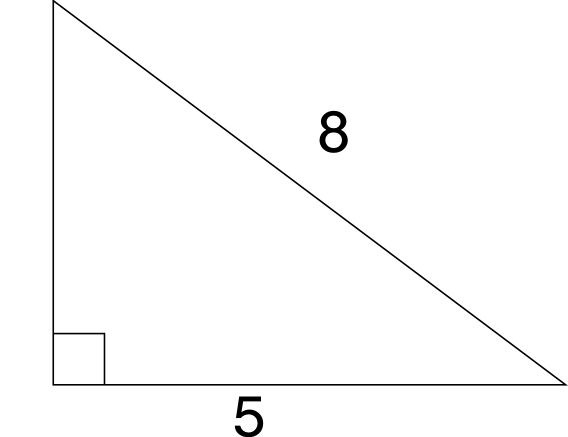
\includegraphics[width=10em]{ink/trigSubs/triangleValuesBottomHyp}
    \vfill
  \item 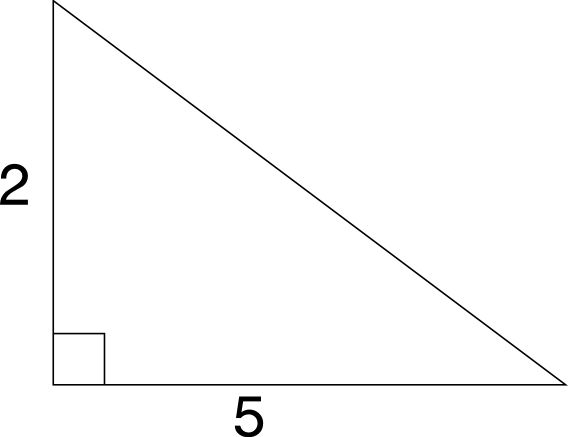
\includegraphics[width=10em]{ink/trigSubs/triangleValuesLeftBottom}
    \vfill
  \item 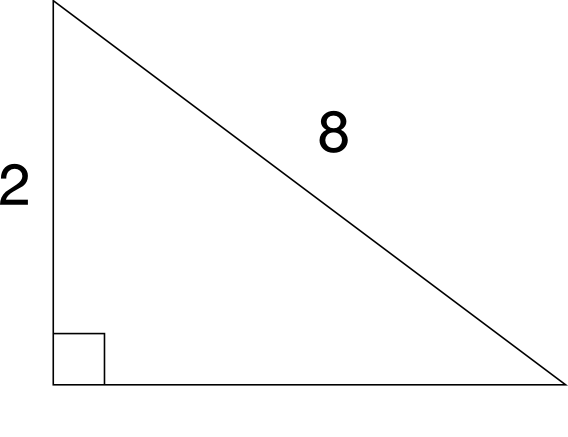
\includegraphics[width=10em]{ink/trigSubs/triangleValuesLeftHyp}
    \vfill
  \end{subproblem}
\end{problem}



\actTitle{Trigonometric Substitution}
\begin{problem}
\item A rod has a charge distribution, and the length of the rod is
  3m. The left endpoint is $x=0$m, and the right endpoint is
  $x=0.5$m. Determine the total charge in the rod for the following
  charge densities.
  \begin{subproblem}
    \item $\lambda_q = \frac{1}{\sqrt{1-x^2}}$ C/m
      \vfill
    \item $\lambda_q = \frac{1}{\sqrt{4-x^2}}$ C/m
      \vfill
  \end{subproblem}
\end{problem}

\postClass

\begin{problem}
\item Briefly state two ideas from today's class.
  \begin{itemize}
  \item
  \item
  \end{itemize}
\item
  \begin{subproblem}
    \item
  \end{subproblem}
\end{problem}


%=========================================================================
% Trig substitutions - day 2
%=========================================================================
\preClass{Integraton}

\begin{problem}
\item For each of the triangles below, determine the length of the
  side with the missing length. Also, determine the sine, cosine, and tangent
    for the angle in the lower right part of the triangle.
  \begin{subproblem}
  \item 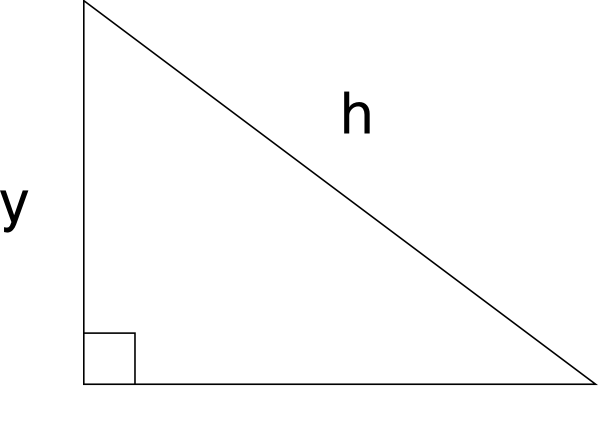
\includegraphics[width=10em]{ink/trigSubs/triangleSymbolsLeftHyp}
    \vfill
  \item 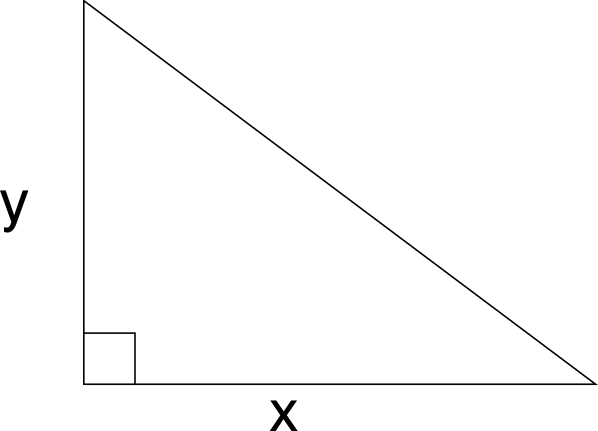
\includegraphics[width=10em]{ink/trigSubs/triangleSymbolsBottomLeft}
    \vfill
  \item 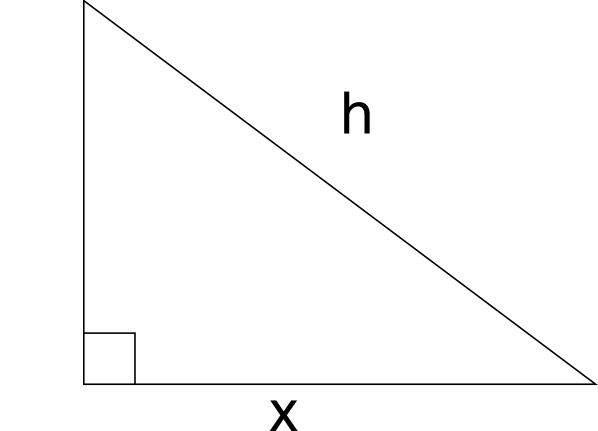
\includegraphics[width=10em]{ink/trigSubs/triangleSymbolsBottomHyp}
    \vfill
  \end{subproblem}
\end{problem}



\actTitle{Trigonometric Substitution}
\begin{problem}
\item A rod has a charge distribution, and the length of the rod is
  3m. The left endpoint is $x=0$m, and the right endpoint is
  $x=3$m. Determine the total charge in the rod for the following
  charge densities.
  \begin{subproblem}
    \item $\lambda_q = \frac{x^2}{\sqrt{1+x^2}}$ C/m
      \vfill
    \item $\lambda_q = \frac{x^2}{\sqrt{4+x^2}}$ C/m
      \vfill
  \end{subproblem}
\end{problem}

\postClass

\begin{problem}
\item Briefly state two ideas from today's class.
  \begin{itemize}
  \item
  \item
  \end{itemize}
\item
  \begin{subproblem}
    \item
  \end{subproblem}
\end{problem}


%=========================================================================
% Start of Volumes of Revolution
%=========================================================================
\preClass{Volumes of Revolution}

\begin{problem}
\item Determine the value of the integral
  \begin{eqnarray*}
    \int^h_0 \pi \left (R-\frac{R}{h} x\right)^2 ~ dx,
  \end{eqnarray*}
  where $h$ and $R$ are constants.
  \vfill

\item What is the volume of a right circular cylinder resting on its
  edge that has a radius of $R$ and a height $h$?

  \vfill

\item What is the volume of two cylinders resting on their edge
  standing next to each other? The first is a right circular cylinder
  that has a radius of $R_1$ and a height $h_1$, and the second is a
  right circular cylinder that has a radius of $R_2$ and a height
  $h_2$.

  \vfill

\end{problem}


\actTitle{Volumes of Revolution}
\begin{problem}
\item Determine the formula for a line that will be revolved
      around the $x$-axis, and the resulting solid will be a right
      circular cone of radius $R$ and height $h$.
  \begin{subproblem}
    \item Make a sketch of the line. (Make an axis and clear mark the
      axes.)
      \vfill

    \item Make a sketch of the resulting solid obtained after
      revolving the line around the $x$ axis.
      \vfill

    \item Determine the integral that represents the volume of the
      cone using washers.
      \vfill

  \end{subproblem}
\end{problem}

\postClass

\begin{problem}
\item Briefly state two ideas from today's class.
  \begin{itemize}
  \item
  \item
  \end{itemize}
\item
  \begin{subproblem}
    \item
  \end{subproblem}
\end{problem}


%=========================================================================
% Start of Volumes of Revolution
%=========================================================================
\preClass{Volumes of Revolution}

\begin{problem}
\item Determine the value of the integral
  \begin{eqnarray*}
    \int^R_0 2\pi x \left( R-x \right) ~ dx.
  \end{eqnarray*}
  \vfill

\item What is the volume of a right circular cylinder that has a
  radius of $R$ and a height $h$ that is resting on its base?

  \vfill

\item What is the volume of two cylinders stacked on top of one
  another vertically? The first is a right circular cylinder that has a radius of
  $R_1$ and a height $h_1$, and the second is a right circular cylinder that
  has a radius of $R_2$ and a height $h_2$.

  \vfill

\end{problem}


\actTitle{Volumes of Revolution}
\begin{problem}
\item Determine the formula for a line that will be revolved
      around the $y$-axis, and the resulting solid will be a right
      circular cone of radius $R$ and height $h$.
  \begin{subproblem}
    \item Make a sketch of the line. (Make an axis and clear mark the
      axes.)
      \vfill

    \item Make a sketch of the resulting solid obtained after
      revolving the line around the $y$ axis.
      \vfill

    \item Determine the integral that represents the volume of the
      cone using shells.
      \vfill

  \end{subproblem}
\end{problem}

\postClass

\begin{problem}
\item Briefly state two ideas from today's class.
  \begin{itemize}
  \item
  \item
  \end{itemize}
\item
  \begin{subproblem}
    \item
  \end{subproblem}
\end{problem}



%=========================================================================
% Start of Areas of Revolution
%=========================================================================
\preClass{Area of Revolution}

\begin{problem}
\item Determine the area of the sector of a circle shown below in
  terms of
  $\theta$ and $R$. \\
  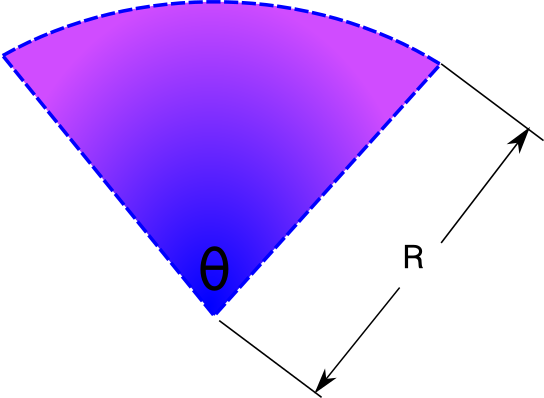
\includegraphics[width=12em]{ink/revolution/sector}

\item Determine the area of the slice of a sector shown below in terms of
  $\theta$, $L_1$, and $L_2$. \\
  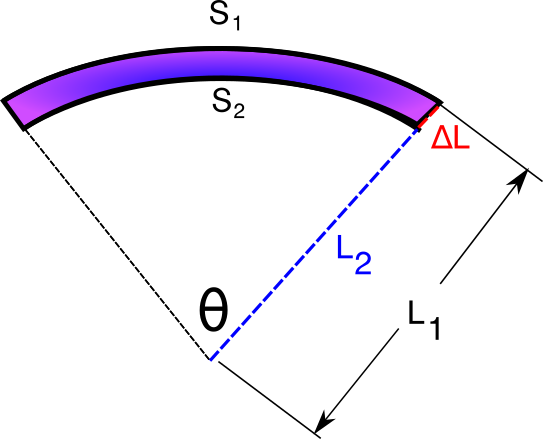
\includegraphics[width=12em]{ink/revolution/sectorDifference}

\item Use the relationship $L_2+\triangle L=L_1$ to express the area
  of the strip in terms of $\theta$, $\triangle L$, and  $L_2$.
  Expand and simplify the result.
  \label{problem:revol:area}
  \vfill

\item Substitute  $L_2\theta=S_2$  into the expression
  for the area in part \ref{problem:revol:area}.

  \vfill

\item Show that ${S_1-S_2}= \triangle L \theta$.

  \vfill


\item Substitute the expression found for $\triangle L \theta$ in the
  expression for the area. Simplify your result, and you should have a
  formula for the area of the strip only in terms of $S_1$, $S_2$, and
  $\triangle L$.

  \vfill

  \sideNote{Hint: $\triangle L^2\theta = \triangle L \cdot \triangle L \theta$}


\end{problem}


\actTitle{Area of Revolution}
\begin{problem}
\item Determine the formula for a line that will be revolved
      around the $x$-axis, and the resulting solid will be a right
      circular cone of radius $R$ and height $h$.
  \begin{subproblem}
    \item Make a sketch of the line. (Make an axis and clear mark the
      axes.)
      \vfill

    \item Make a sketch of the resulting solid obtained after
      revolving the line around the $y$ axis.
      \vfill

    \item Determine the integral that represents the area of the cone.
      \vfill

  \end{subproblem}
\end{problem}

\postClass

\begin{problem}
\item Briefly state two ideas from today's class.
  \begin{itemize}
  \item
  \item
  \end{itemize}
\item
  \begin{subproblem}
    \item
  \end{subproblem}
\end{problem}


%=========================================================================
% Start of partial fractions
%=========================================================================
\preClass{Rational Functions}

\begin{problem}
\item Express each function below as a single fraction. That is bring
  the two parts together over a common denominator and simplify the
  result.
  \begin{subproblem}
  \item $\frac{1}{x+3} + \frac{1}{x+2}$
    \vfill
  \item $\frac{1}{x+3} + \frac{3}{x-2}$
    \vfill
  \item $\frac{1}{x+3} + \frac{4}{x-3}$
    \vfill
  \end{subproblem}
\end{problem}


\actTitle{Partial Fractions}
\begin{problem}
\item Determine the common denominator for each of the expressions below.
  \begin{subproblem}
    \item $\frac{1}{x} + \frac{1}{x-3}$ \\
      Common Denominator: \framebox(250,50){~}
      \vfill
    \item $\frac{8}{x+7} + \frac{20}{x+50}$ \\
      Common Denominator: \framebox(250,50){~}
      \vfill
    \item $\frac{8,250}{x+7} + \frac{x}{x+50}$ \\
      Common Denominator: \framebox(250,50){~}
      \vfill
  \end{subproblem}

  \clearpage

\item For each of the following functions write the general form of
  the partial fraction expansion. The first one is completed as an
  example.
  \begin{subproblem}
    \item $\frac{2x+1}{x^2+2x-8}$ \\
      General Form: \framebox(250,50){$\frac{A}{x+4} + \frac{B}{x-2}$}
      \vfill
    \item $\frac{8x+1}{x^2-x-12}$ \\
      General Form: \framebox(250,50){~}
      \vfill
    \item $\frac{5x-10}{x^2-16}$ \\
      General Form: \framebox(250,50){~}
      \vfill
    \item $\frac{4x+2}{x^2-5x}$ \\
      General Form: \framebox(250,50){~}
      \vfill
  \end{subproblem}

\end{problem}

\postClass

\begin{problem}
\item Briefly state two ideas from today's class.
  \begin{itemize}
  \item
  \item
  \end{itemize}
\item
  \begin{subproblem}
    \item
  \end{subproblem}
\end{problem}


\preClass{Rational Functions}

\begin{problem}
\item Express each function below as a single fraction. That is bring
  the two parts together over a common denominator and simplify the
  result.
  \begin{subproblem}
  \item $\frac{1}{x+2} + \frac{3}{(x+2)^2}$
    \vfill
  \item $\frac{1}{x+3} + \frac{2}{(x+3)^2}$
    \vfill
  \item $\frac{1}{x} + \frac{1}{x^2} + \frac{1}{x^2}$
    \vfill
  \end{subproblem}
\end{problem}

\actTitle{Partial Fractions}
\begin{problem}
\item Determine the common denominator for each of the expressions below.
  \begin{subproblem}
    \item $\frac{1}{x-3} + \frac{1}{x^2-6x+9}$ \\
      Common Denominator: \framebox(250,50){~}
      \vfill
    \item $\frac{8}{x+7} + \frac{20}{x^2+14x+49}$ \\
      Common Denominator: \framebox(250,50){~}
      \vfill
    \item $\frac{8,250}{x+7} + \frac{x}{x^2+14x+49}$ \\
      Common Denominator: \framebox(250,50){~}
      \vfill
  \end{subproblem}

  \clearpage

\item For each of the following functions write the general form of
  the partial fraction expansion. The first one is completed as an
  example.
  \begin{subproblem}
    \item $\frac{2x+1}{x^2+2x-8}$ \\
      General Form: \framebox(250,50){$\frac{A}{x+4} + \frac{B}{x-2}$}
      \vfill
    \item $\frac{8x+1}{x^2-x-12}$ \\
      General Form: \framebox(250,50){~}
      \vfill
    \item $\frac{5x-10}{x^2+8x+16}$ \\
      General Form: \framebox(250,50){~}
      \vfill
    \item $\frac{4x+2}{x^2-10x+25}$ \\
      General Form: \framebox(250,50){~}
      \vfill
  \end{subproblem}

\end{problem}


\postClass

\begin{problem}
\item Briefly state two ideas from today's class.
  \begin{itemize}
  \item
  \item
  \end{itemize}
\item
  \begin{subproblem}
    \item
  \end{subproblem}
\end{problem}


\preClass{Rational Functions}

\begin{problem}
\item For each of the quadratic functions below complete the square to
  express each function in the form
  \begin{eqnarray*}
    f(x) & = & A(x-B)^2 + C.
  \end{eqnarray*}
  \begin{subproblem}
  \item $x^2 - 2x + 2$
    \vfill
  \item $x^2 - 6x + 12$
    \vfill
  \item $2x^2 - 4x + 6$
    \vfill
  \end{subproblem}
\end{problem}

\actTitle{Partial Fractions}
\begin{problem}
\item For each integral below complete the square on the denominator
  and then use $u$-substitution to determine the integral.
  \begin{subproblem}
    \item ${\displaystyle \int}\frac{1}{x^2 - 2x + 2}~dx$ \\
      \vfill
    \item ${\displaystyle\int}\frac{2}{x^2 - 6x + 12}~dx$ \\
      \vfill
    \item ${\displaystyle\int}\frac{1}{x^2 + 8x + 26}~dx$ \\
      \vfill
  \end{subproblem}

  \clearpage

\item Determine the value of the integral
  \begin{eqnarray*}
    \int \frac{1}{x^3+x^2+3\,x-5} ~ dx
  \end{eqnarray*}

  \vfill

\end{problem}


\postClass

\begin{problem}
\item Briefly state two ideas from today's class.
  \begin{itemize}
  \item
  \item
  \end{itemize}
\item
  \begin{subproblem}
    \item
  \end{subproblem}
\end{problem}





%%% Local Variables:
%%% mode: latex
%%% TeX-master: t
%%% End:
